\chapter{Iteración 5}
\section{Objetivos de iteración}
\begin{itemize}
  \item Definición de API en Swagger
  \item Implementación inicial de API REST
  \item Primeros tests
  \item Despliegue en plataforma Azure
  \item Investigar integración contínua
\end{itemize}


\section{Definición de API en Swagger}
TODO URL a Swagger y a wiki de projetsii, etc


\section{Implementación inicial de API REST}
TODO Contar algo de SessionController, SessionsController y la API


\section{Primeros tests}
TODO  Contar qué tests hay, más o menos.


\section{Despliegue en plataforma Azure}
Tras evaluar las opciones de despliegue de \emph{Docker} en \emph{Azure} hemos
optado por construir una máquina virtual donde administraremos manualmente una
instancia de \emph{Docker} en vez de utilizar la extensión de máquina virtual
que implementa \emph{Azure} para \emph{Docker}. Utilizar esta última habría implicado
una complejidad añadida por la parafernalia necesaria para mantener certificados de
seguridad para poder comunicarnos con la instancia de  \emph{Docker}.

En lugar de la extensión de máquina virtual de \emph{Azure} administraremos la 
máquina virtual manualmente.


\subsection{Test vm}
Para esta iteración hemos creado una máquina virtual cuyo propósito es familiarizarnos
con el entorno \emph{Azure}. Para ello los requisitos de esta máquina serían:

\begin{itemize}
 \item Ser capaz de ejecutar el servidor \emph{GameRegistry} y \emph{MongoDB} como
       contenedores de \emph{Docker}.
 \item Ser capaz de construir el contenedor de \emph{GameRegistry} a partir del 
       repositorio SVN del proyecto.
\end{itemize}

Para ello se ha basado la máquina virtual en una imagen de \emph{Ubuntu 15.04}, que contiene
una versión reciente y razonablemente testada de \emph{Docker}. Además hemos añadido
el cliente de \emph{Subversion} y el \emph{OpenJDK-8}.


\subsection{VM de producción}
Aún no creada. Sus requisitos son similares pero no iguales a la máquina test. El propósito
de esta máquina virtual será el de ejecutar el servidor, evitando la instalación
de cualquier pieza de software no necesaria para esa tarea, lo cual en este caso implica
no instalar ningún \emph{JDK} ni \emph{Subversion}.

Esto requiere algún método para hacer llegar el contenedor con el servidor GameRegistry a
la máquina que no implique a \emph{Subversion} ni el uso de \emph{Java} para compilar
el código fuente. Lo resolveremos en la próxima iteración.

\begin{figure}[h]
 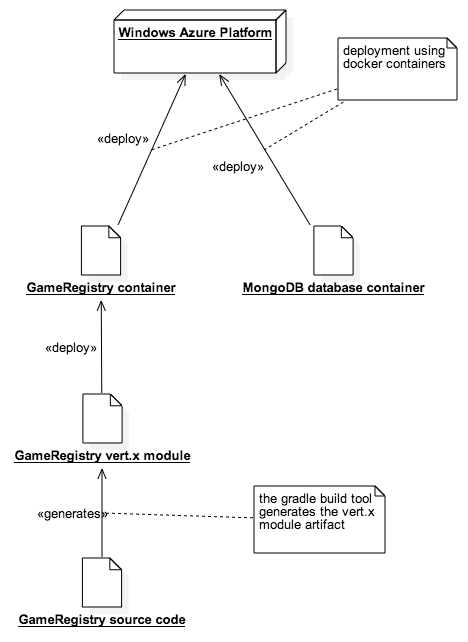
\includegraphics[scale=0.6]{diagrams/docker_deployment_diagram.png}
 \caption{Diagrama de despliegue (iteración 5)}
 \label{fig:despliegue}
\end{figure} 


\section{Investigar integración contínua}
Algún método de integración contínua sería interesante para el proyecto de forma que los tests 
sean ejecutados en cada revisión del proyecto. Hay sitios web que ofrecen una instancia gratuita de
integración contínua que podrían ser utilizados, como por ejemplo:

\begin{itemize}
\item CircleCI (\texttt{https://circleci.com/})
\item CodeShip (\texttt{https://codeship.com/})
\end{itemize}

Estamos aún estudiando la viabilidad y los requisitos impuestos.